\section{Project description}
\begin{frame}{Grasp of thin objects}
  \begin{columns}
    \begin{column}{0.5\textwidth}
      VIDEO PROBLEM
    \end{column}
    \begin{column}{0.5\textwidth}
      \begin{alertblock}{Problem}
        Performing the grasp of thin objects could be a hard task
        because not enough contact constraints are provided by the object
      \end{alertblock}
    \end{column}
  \end{columns}
\end{frame}

\begin{frame}{A solution to the problem}
  Use of environmental constraints to arrange an easier grasp and
  then perform the grasp
  \begin{columns}
    \begin{column}{0.5\textwidth}
      \vskip+0.1in
      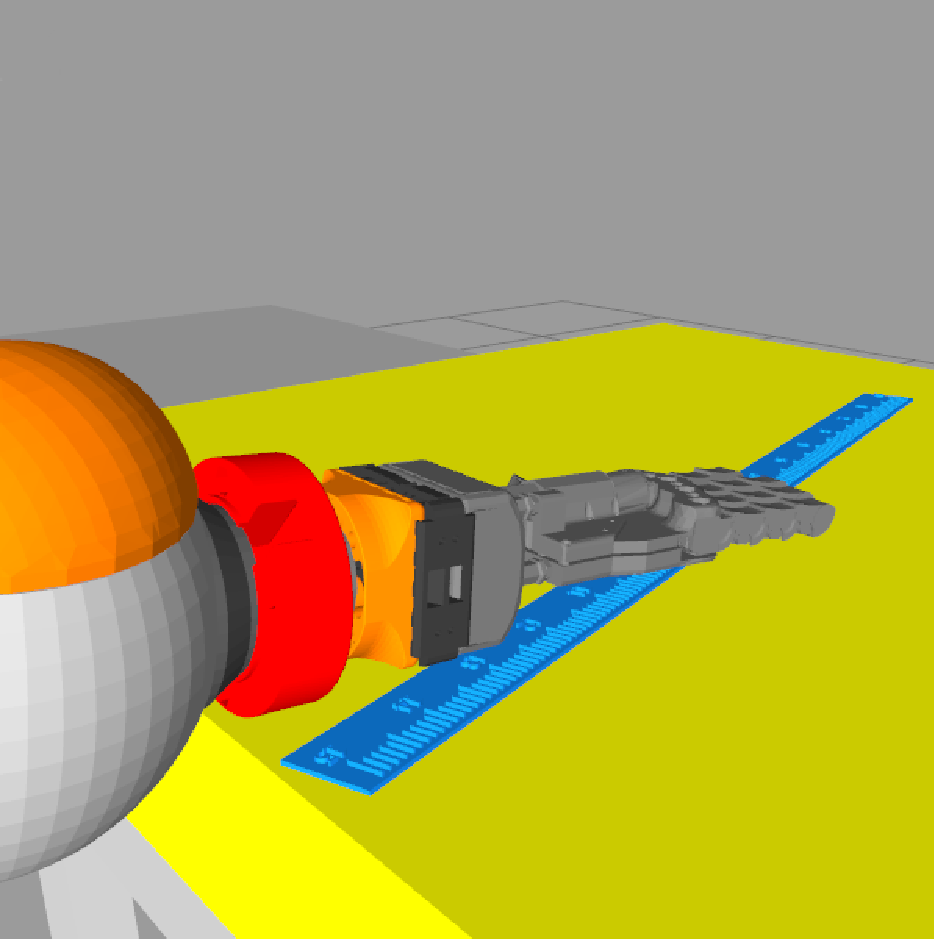
\includegraphics[width=\columnwidth]{hand_on_ruler}
    \end{column}
    \begin{column}{0.5\textwidth}
      \begin{exampleblock}{Example}
        \begin{itemize}
        \item[1.] the hand is placed on the object
        \item[2.] the hand drags the object until it \alert{sticks out 
          of the border} of the table 
        \item[3.] the hand grasps the object
        \end{itemize}
      \end{exampleblock}
    \end{column}
  \end{columns}
\end{frame}

\begin{frame}{How to perform a safe dragging phase}
  The dragging phase could \alert{damage} the object due to uncontrolled contact forces between the 
  hand and the object.
  \par
  An hybrid position force control strategy allows to avoid this issue.
  \vskip0.5in
  \begin{exampleblock}{Aim of this project}
    Develop an hybrid force position control that allows to move the hand and 
    at the same time to regulate the contact force using a force feedback signal.
  \end{exampleblock}
\end{frame}
